\documentclass{article}
\usepackage{graphicx}

\author{Meftah, Morteza M.D,; Waren, Daniel M.D; Bosco, Joseph A. IV;\\
Di Gangi, Catherine; Watson, Cody Ph.D}
\title{Modeling Robotic Surgery Predictions: Write-Up}

\begin{document}

\maketitle

\begin{figure}[h]
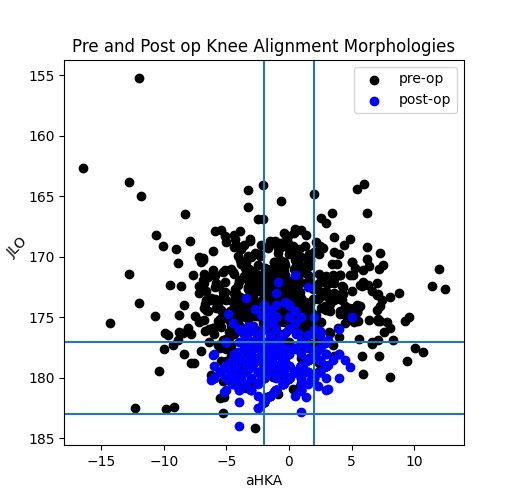
\includegraphics[width=.9\textwidth]{data_vis.png}
\caption{These are the averages of the clusters. }
\end{figure}



\newpage

\begin{figure}[h]
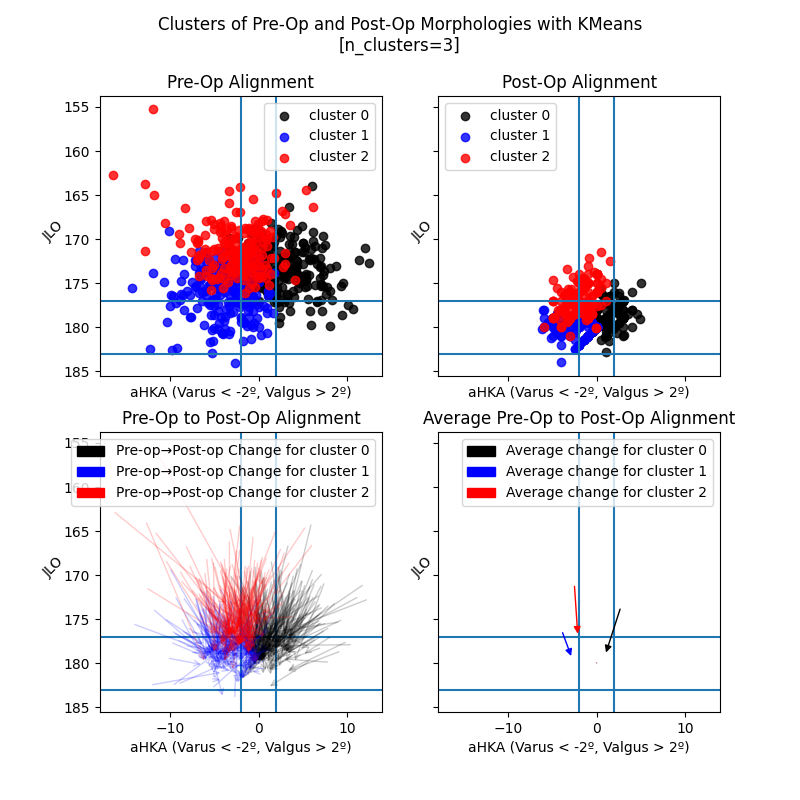
\includegraphics[width=\textwidth]{clusters.png}
\caption{These are the clusered data points.}
\end{figure}

\begin{figure}[h]
	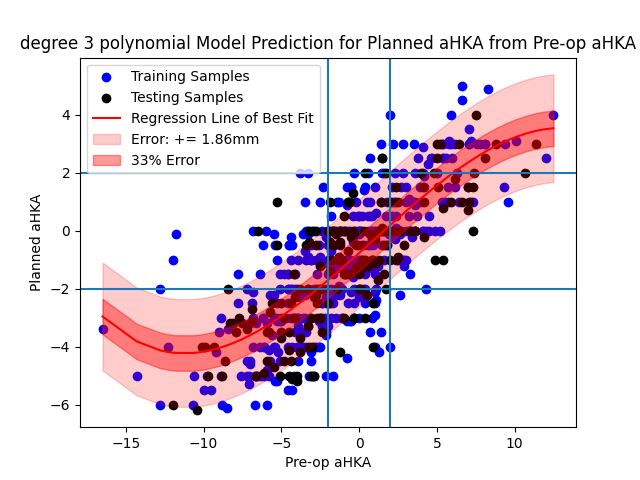
\includegraphics[width=\textwidth]{degree_3_polynomial_regression.png}
	\caption{This is a regression trained using a linear regression algorithm.
	The error is the mean squared distance from the testing set (black). 
	The regression is trained on the training set (blue)}
\end{figure}


\begin{figure}[h]
	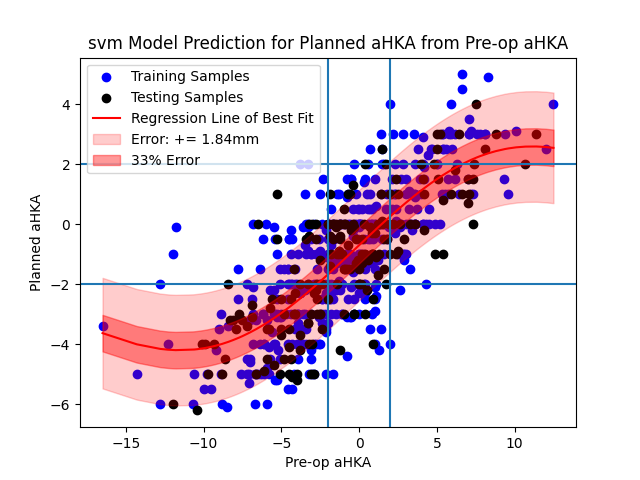
\includegraphics[width=\textwidth]{svm_regression.png}
	\caption{This is a regression trained using a support vector machine algorithm.
	The error is the mean squared distance from the testing set (black). 
	The regression is trained on the training set (blue)}
\end{figure}

\begin{figure}[h]
	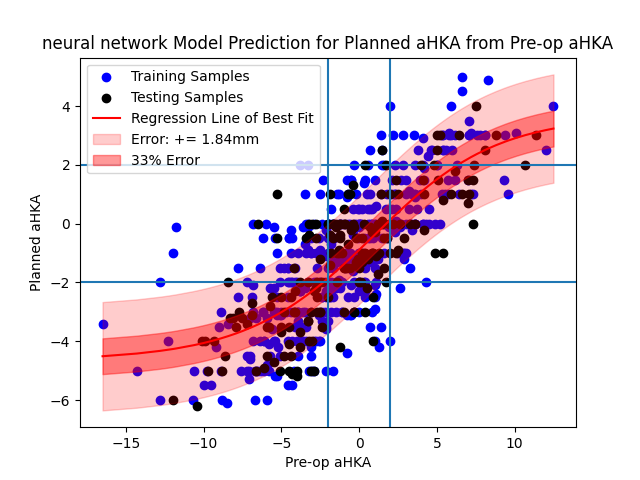
\includegraphics[width=\textwidth]{neural_network_regression.png}
	\caption{This is a regression trained using a deep learning algorithm on a MLP/neural network model.
	The error is the mean squared distance from the testing set (black). 
	The regression is trained on the training set (blue)}
\end{figure}

\end{document}

